\documentclass{scrartcl}

% So that TeX doesn't complain about small
% underfull or overfull boxes
\hfuzz1pc
% Make the overfull marker bigger
\overfullrule=2cm

% Font setup.
\usepackage{unicode-math}
\setmainfont{STIX Two Text}
\setsansfont[Scale=MatchLowercase]{Source Sans 3}
\setmonofont[Scale=MatchLowercase]{Ubuntu Mono}
\setmathfont[Scale=.93]{STIX Two Math}
\linespread{1.05}
% Don't put extra space after periods
\frenchspacing
\KOMAoptions{
    paper = letter,
    BCOR = 0mm,
    twoside = false,
    fontsize = {8},
    DIV = calc,
}

% Make bibliography more compact, no indents.
\KOMAoption{toc}{flat}

% Language support, usually changes between english
% and spanish.
\usepackage[spanish,es-noindentfirst]{babel}
%\usepackage[english]{babel}
\usepackage{csquotes}

% Bibliography
\usepackage[
    backend=biber,
    style=numeric-comp,
    backref=true,
    backrefstyle=two,
    abbreviate=true
]{biblatex}
\addbibresource{~/git/Misc-LaTeX-files/bib/general.bib}
\addbibresource{~/git/Misc-LaTeX-files/bib/math-books.bib}

% Graphics, mainly to insert images or
% single page PDFs.
\usepackage{graphicx}
\usepackage[dvipsnames]{xcolor}
% Handy command to typeset URLs
\usepackage{hyperref}
\hypersetup{
    colorlinks=true,
    linkcolor=Mahogany,
    filecolor=Mahogany,
    urlcolor=Black,
    citecolor=Mahogany,
}
\usepackage{url}
%\urlstyle{same}
\usepackage{metalogo}

%\usepackage{minted}

% Font style and size for title
\setkomafont{title}{\itshape}
% Font style for the subject
\setkomafont{subject}{\normalfont}
% Font style for subtitle
\setkomafont{subtitle}{\normalfont\itshape}
\setkomafont{author}{\large}
\setkomafont{date}{\normalsize}
\setkomafont{section}{\fontseries{m}\Large}
\setkomafont{subsection}{\fontseries{m}\large}
\setkomafont{subsubsection}{\fontseries{m}\normalsize}

% Footnotes
\deffootnote{2.0em}{1.5em}{\thefootnotemark.\ }
\setkomafont{footnote}{\sffamily}

\newcounter{exer}
\newcommand{\exercise}{%
    \stepcounter{exer}%
    \begin{center}%
        \addfontfeatures{LetterSpace=7}\large\Roman{exer}%
    \end{center}%
}
\newcommand{\solution}{
    \begin{center}
        Solución
    \end{center}
}

% CUSTOM MACROS
% math macros
\renewcommand{\Rn}{\mathbb{R}^{\mathrm{n}}}
\newcommand{\Rm}{\mathbb{R}^{\mathrm{m}}}
\newcommand{\R}{\mathbb{R}}
\newcommand{\N}{\mathbb{N}}
\newcommand{\devpart}[2]{\frac{\partial  #1}{\partial #2}}
\renewcommand{\vec}[1]{\mathbf{#1}}
\newcommand{\norm}[1]{\left\lvert #1 \right\rvert}
\newcommand{\iprod}[2]{\left\langle #1 , #2 \right\rangle}
\newcommand{\devp}[2]{\frac{\partial #1}{\partial #2}}
\DeclareMathOperator{\img}{img}
\DeclareMathOperator{\gen}{span}


\begin{document}
%
\title{Tercera Tarea}
\subtitle{Cadenas de markov}
\subject{Aplicación a los procesos estocásticos discretos}
\titlehead{Universidad Simón Bolívar\hfill Caracas, Venezuela}
\author{Jhonny Lanzuisi}
\date{\today}
\maketitle

\setcounter{exer}{3}
\exercise
Una partícula se mueve a través de los estados 0, 1 y 2 de acuerdo
a un proceso Markoviano cuya matriz de transición es:
\[
	P = \begin{pmatrix}
		0 & 1/2 & 1/2 \\
		1/2 & 0 & 1/2 \\
		1/2 & 1/2 & 0 \\
	\end{pmatrix}	
\]

Sea $X_n$ la posición de la partícula en el $n$-ésimo movimiento.
Calcule $\Prob(X_n = 0\mid X_0 = 0)$ para
$n = 0, 1, 2, 3, 4$. ¿Qué puede decir al respecto?

\solution
Para calcular las probabilidades pedidas hace falta conocer las
potencias de $P$ hasta $P^4$.

\begin{gather*}
	P^2 = \begin{pmatrix}
		1/2 & 1/4 & 1/4 \\
		1/4 & 1/2 & 1/4 \\
		1/2 & 1/2 & 1/4
	\end{pmatrix}
	\quad
	P^3 = \begin{pmatrix}
		1/4 & 3/8 & 3/8 \\
		3/8 & 1/4 & 3/8 \\
		3/8 & 3/8 & 1/4
	\end{pmatrix} \\
	P^4 = \begin{pmatrix}
		3/8 & 5/16 & 5/16 \\
		5/16 & 3/8 & 5/16 \\
		5/16 & 5/16 & 3/8
	\end{pmatrix}
\end{gather*}

Ahora, las entradas $(0,0)$ de la matriz nos dicen las probabilidades
que buscamos:
\begin{align*}
	\Prob(X_0 = 0\mid X_0 = 0) &= P^0(0,0) = I(0,0) = 1\\
	\Prob(X_1 = 0\mid X_0 = 0) &= P^1(0,0) = 0\\
	\Prob(X_2 = 0\mid X_0 = 0) &= P^2(0,0) = 1/2\\
	\Prob(X_3 = 0\mid X_0 = 0) &= P^3(0,0) = 1/4\\
	\Prob(X_4 = 0\mid X_0 = 0) &= P^4(0,0) = 3/8.
\end{align*}

\setcounter{exer}{8}
\exercise
Considere la cadena de Markov con espacio de estados 
$E = \{0, 1, 2, 3\}$ y matriz de transición dada por
\[
	P = \begin{pmatrix}
		1 & 0 & 0 & 0\\
		0.1 & 0.2 & 0.5 & 0.2\\
		0.1 & 0.2 & 0.6 & 0.1\\
		0 & 0 & 0 & 1
	\end{pmatrix}	
\]

Comenzando en el estado $1$, determine la probabilidad de que el proceso sea absorbido por el estado
$0$. Compare esto con la $(1, 0)$-ésima entrada de las potencias de matrices $P^2$ , $P^4$ , $P^8$ y $P^{16}$

\clearpage
\solution
Sea $h_i = \Prob(\text{llegar al 0, partiendo del estado $i$})$.
Las probabilidades de llegar al estado cero partiendo de los otros estados
vienen dadas por el siguiente sistema linear.
\[
	\begin{cases}
		h_0 = 1\\
		h_1 = (0.1)h_0 + (0.2)h_1 + (0.5)h_2 + (0.2)h_3\\
		h_2 = (0.1)h_0 + (0.2)h_2 + (0.6)h_2 + (0.1)h_3\\
		h_3 = 0
	\end{cases}	
\]

Las soluciones del sistema anterior son $h_2=0.455$ y $h_1 = 0.409$.
Las $(1,0)$-ésimas entradas de las potencias de $P$ son:
\[P^2(1,0) = 0.17,\; P^4(1,0) = 0.27,\; P^8(1,0) = 0.36,\; P^{16}(1,0) = 0.40.\]

La expresión anterior parece indicar que las coordenadas  $(1,0)$-ésimas
de las potencias de $P$ que son potencias de $2$ tienden a $h_1$.

\setcounter{exer}{6}
\exercise
Sea $\mathcal{X}$ una cadena de Markov con espacio de estados 
$E = {1,\dots,10}$ y matriz de transición $P$ (ver enunciado original).

\solution
En la figura 1 esta un grafo en el que $i\rightarrow j$ significa que $f_{ij}>0$.

\begin{figure}
	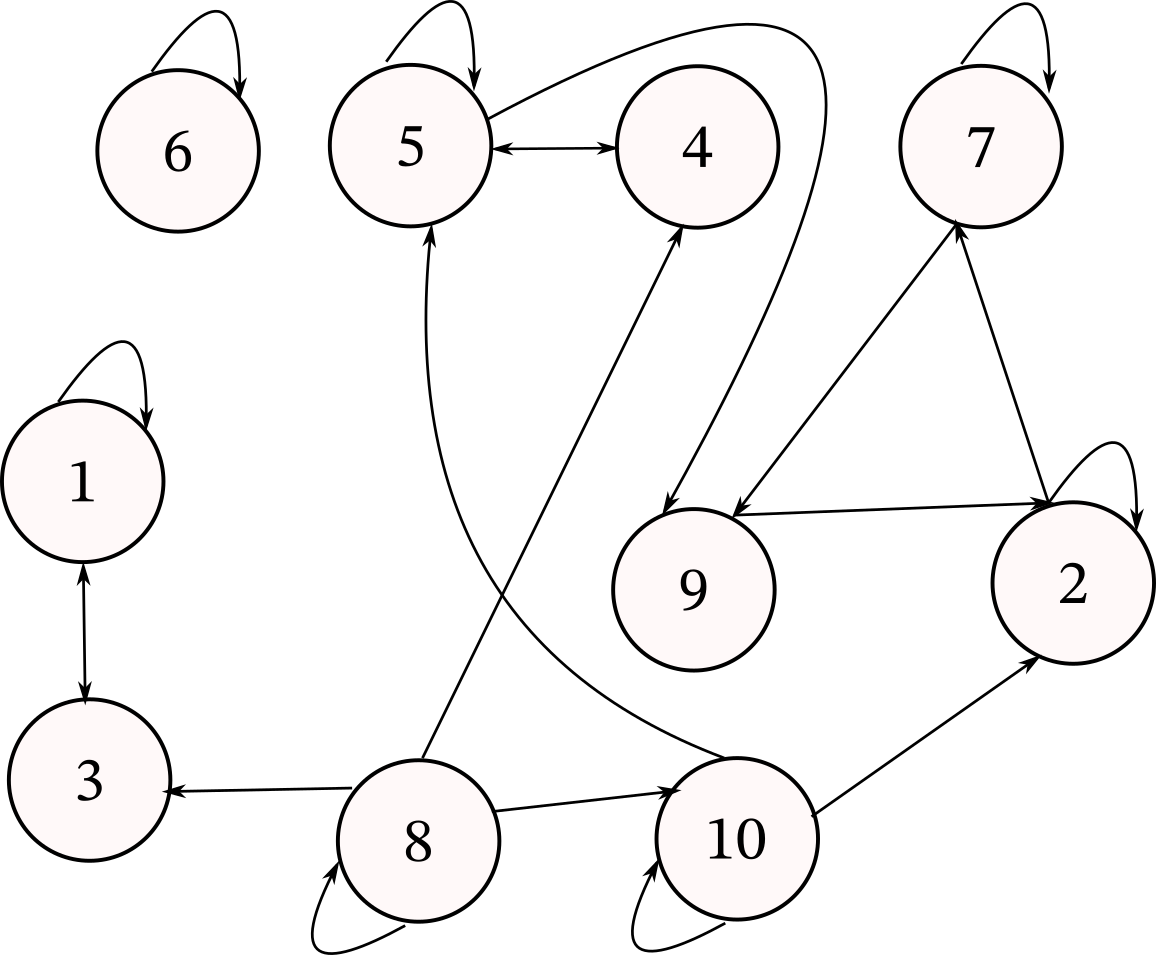
\includegraphics[width=\textwidth]{fig1.png}
	\caption{Grafo ejercicio 7}
\end{figure}

\newpage
\section*{Colophon \& Copyright}
This document was typeset using \TeX%
\footnote{%
    \TeX\ is
    a typesetting software, free and open source,
    developed by Donald Knuth. \LaTeX\ is a macro
    set for \TeX\ developed by Leslie Lamport. \LuaTeX\ is
    a reworking of \TeX\ adding native support for the Lua
    programming language and unicode, among other things.
    All of them are available in all major
    operating systems.
}
and the \LaTeXe\ macros in a GNU/Linux system.
The editor used for editing the text was Visual Studio Code.%
The main typeface used is the STIX Two family%
\footnote{%
    The STIX typefaces were design for technical typesetting,
    and they include both text and math fonts.
}
for text and math,
the sans-serif typeface is Source Sans by Adobe%
\footnote{%
    This is a free and open source typeface comissioned by Adobe.
}.

\medskip
%
\begin{quote}
\sffamily\small
     E-mail: \url{jalb97@gmail.com}. \\
    Copyright (C) 2021 Jhonny Lanzuisi. \\
    This work is licensed under the Creative Commons Attri\-bu\-tion-Sha\-re\-Alike
    International (CC BY-SA 4.0)  License. To view a copy of the license,
    visit \url{https://creativecommons.org/licenses/by-sa/4.0/}.
\end{quote}

\end{document}